\documentclass[11pt,a4paper]{article}
\usepackage{ifpdf}
\usepackage[utf8]{inputenc} \usepackage[francais]{babel}
\usepackage[T1]{fontenc} \usepackage[nottoc, notlof, notlot]{tocbibind}
\usepackage[unicode=true,pdftex,colorlinks=true,linkcolor=black,urlcolor=black,citecolor=black]{hyperref}
\usepackage{natbib}
\usepackage{graphicx}

\parindent 0.8cm
% \setlength{\parskip}{0.5em plus 0.2em minus 0.2em}

\title{Projet Androïd : Rapport}
\author{Anthony \textsc{Caillaud} Manoël \textsc{Fortun} Vincent
\textsc{Pottier} Charles \textsc{Dejean}}
\date{\today}
\ifpdf \pdfinfo { /Author (Anthony Caillaud Manoël Fortun Vincent Pottier
Charles Dejean) /Title (RoadMapJDR) /Subject (RoadMapJDR) /Keywords ()
/CreationDate (D:20100329212218) } \fi


\begin{document}

\maketitle

\clearpage \tableofcontents \clearpage
\section{Introdution}

Ce rapport reprend la suite de la Roadmap que nous avions défini pour notre
projet d'ihm autour d'une application pour jeux de rôles sous androïd. Dans la
continuité du précédent rapport, nous avons suivi la méthode LUCID pour la
conception et réalisation de notre application. Ce rapport reprendra donc à
l'étape 2 de LUCID et finira à l'étape 6 avec le plan d'évaluation, effectif si
nous étions dans un contexte réel. Avant chaque étape, nous rappelerons les
enjeux de celle-ci et notre interprétation.

\clearpage

\section{Lucid 2}

\subsection{Définition}

Cette étape de la méthode permet de compléter la RoadMap. Elle indique les
attentes des utilisateurs receuillies en fonction des catégories d'utilisateur
et du concept de l'application. Elle nous permet aussi de connaître les
fonctionnalités qu'ils jugent indispensables, la façon qu'ils auraient
d'appréhender l'application via des scénarios.

\subsection{Approche des utilisateurs}

Nous avons soumis notre projet à des rôlistes, pas tous experts en
informatique. Le cliché des geeks informaticiens rôlistes est loin d'être une
vérité! Nous n'avons pas eu besoin de partitionner les résultats et de
les analyser séparément en fonction des catégories d'utilisateurs.\\

De plus, nous avons pensé qu'interroger des gens qui ne connaissent pas le jeu
de rôle mais connaissant l'informatique ou les applications mobiles n'était pas
pertinent. En effet, séduire des gens "experts" en mobile au jeu de rôle n'est
pas le but de l'application. Cette partie de l'étude n'a donc pas été menée.
C'est peut-être un biais que nous n'aurions pas dû prendre, mais l'intérêt nous
semblait très limité.\\

Dans notre approche de l'étude des commentaires de futurs utilisateurs, nous
nous sommes rendu compte que nos explications n'étaient pas toujours
claires. En effet, certains premiers "clients" nous ont demandé si nous n'étions
pas en train de faire un jeu! Par la suite, nous avons mieux construis nos
explications.\\

Dans les réponses que nous avons pu récolter, il y a trois grand types de
réaction commune qui étaient assez prévisible.\\

%%En général les gens trouvent que Joël il est tout petit.\\

La première réaction est celle des irréductibles, accrochés à la symbolique du
support physique de leurs dés et de leurs fiches. "Parce que lancer un
téléphone sur un joueur c'est quand même plus onéreux que lui lancer ses dés"!\\

Ensuite il y a les gens très enthousiaste par l'idée. Les joueur et les MJ sont
intéressés et souhaitent voir des choses comme la synchronisation facile avec
un ordinateur ou encore des thèmes personnalisables en fonction du jeu. De
plus, ils exprimaient aussi le fait d'avoir des dés visuels et personnalisable
eux aussi.\\

Enfin, il y a les gens curieux de voir ce que l'application va être et de
voir ce qu'elle apportera à leur manière de jouer.\\

Une fois ces premières réactions généralistes analysées, il y a quelques
demandes particulières. Tout d'abord, le fait de pouvoir convertir ses fiches en
fiches papiers imprimables et pré-remplies. Ensuite, la partie connectivité qui
à été compliqué à expliquer tant elle est à la fois proche et éloignée d'un
système de chat classique. Ce qui se ressent, c'est le sentiment d'espionnage
par le MJ.\\

Au niveau IHM pur et concept lié, les gens ont tendance à penser que le support
téléphone tout en étant pratique est moins adapté qu'une tablette graphique.
Convaincre avec cette application peut être compliqué. Nous avons pu nous rendre
compte par cette étude menée autour de parties et dans la façon qu'ont les
joueurs d'utiliser leur fiche que la navigation entre différents niveaux d'une
fiche doit être rapide et simple. De même, les éditions de certains composants
de personnage comme son niveau de vie doivent être très rapide cette
modification arrive souvent au cours d'une partie.\\

Celà nous à permis de compléter les UserStories que nous avions déjà commencé à
définir.\\

\subsection{User Stories}

Cette partie regroupe donc nos scénarios construits en partie en amont de la
phase de communication et complétés après analyse des réactions clients.

\chapter{User Stories pour le composant dé}

En tant que Joueur, avec le composant de dés, je dois pouvoir lancer un nombre
de dé choisi et du type que je souhaite et je dois pouvoir voir le résultat
correct.
~

En tant que Joueur, avec le composant de dés, je dois pouvoir, après un jet de
dés, relancer les dés avec les mêmes caractéristiques.
~

En tant que Joueur, avec le composant de dés, je dois pouvoir changer le type de
dés ou le nombre

\clearpage


\subsubsection{User Stories pour la connectivité}

En tant que Joueur, avec le module Connectivité, je dois pouvoir rejoindre une
salle de chat.\\

En tant que Joueur, avec le module Connectivité, je dois pouvoir créer un salon
et devenir maître de salon.\\

En tant que Joueur, avec le module Connectivité, je dois pouvoir parler de façon
discrète (privée) à un autre joueur présent.\\

En tant que Joueur, avec le module Connectivité, je dois pouvoir choisir que
toutes mes conversations soient visibles par le maître de salon.\\

En tant que Joueur, avec le module Connectivité, je dois pouvoir choisir que
tous mes jets soient envoyés au Maître du salon.\\


En tant que Maître du salon, avec le module Connectivité, je dois pouvoir
choisir de ne pas voir les conversations ou les dés.\\

En tant que Joueur, avec le module Connectivité, je dois pouvoir ne pas être que
sur un salon.\\

En tant que Joueur, avec le module Connectivité, je dois pouvoir accéder à la
liste des gens sur le salon.\\

En tant que Joueur, avec le module Connectivité, je dois pouvoir, depuis ma
fiche, accéder rapidement au salon ou je suis connecté.\\



\subsubsection{User Stories pour le Joueur}

En tant que Joueur, dans la partie consultation de fiche, je dois pouvoir voir
les caractéristiques du personnage.\\

En tant que Joueur, dans la partie consultation de fiche, je dois pouvoir voir
les compétences du personnage.\\

En tant que Joueur, dans la partie consultation de fiche, je dois pouvoir voir
les autres informations du personnage, en fonction du jeu.\\

En tant que Joueur, dans la partie consultation de fiche, je dois pouvoir voir
les caractéristiques secondaires du personnage.\\

En tant que Joueur, dans la partie consultation de fiche, je dois pouvoir
sélectionner une caractéristique afin de pouvoir la modifier.\\

En tant que Joueur, dans la partie consultation de fiche, je dois pouvoir
sélectionner une compétence afin de pouvoir la modifier.\\

En tant que Joueur, dans la partie consultation de fiche, je dois pouvoir
sélectionner une caractéristique secondaire afin de pouvoir la modifier.\\

En tant que Joueur, dans la partie consultation de fiche, je dois pouvoir
passer d'une catégorie à une autre facilement.\\

En tant que Joueur, dans la partie consultation de fiche, je dois pouvoir
sélectionner la fiche consultée pour une autre partie.\\


\chapter{User Stories pour le MJ}

En tant que MJ, dans la partie fiche de joueurs, je dois pouvoir voir les
caractéristiques d'une feuille de joueur.
~

En tant que MJ, dans la partie fiche de joueurs, je dois pouvoir voir les
compétences d'une feuille de joueur.
~

En tant que MJ, dans la partie fiche de joueurs, je dois pouvoir voir les
caractéristiques secondaires d'une feuille de joueur.
~

En tant que MJ, dans la partie fiche de joueurs, je dois pouvoir voir les
pouvoirs d'une feuille de joueur.
~

En tant que MJ, dans la partie fiche de joueurs, je dois pouvoir voir les
barre de vie d'une feuille de joueur.
~

En tant que MJ, dans la partie fiche de joueurs, je dois pouvoir choisir une
feuille de joueur.
~

En tant que MJ, dans la partie fiche de pnjs, je dois pouvoir choisir une
feuille de pnj. ~

En tant que MJ, dans la partie fiche de pnj, je dois pouvoir voir les
caractéristiques d'une feuille de pnj.
~

En tant que MJ, dans la partie fiche de pnj, je dois pouvoir voir les
compétences d'une feuille de pnj.
~

En tant que MJ, dans la partie fiche de pnj, je dois pouvoir voir les
caractéristiques secondaires d'une feuille de pnj.
~

En tant que MJ, dans la partie fiche de pnj, je dois pouvoir voir les
pouvoirs d'une feuille de pnj.
~

En tant que MJ, dans la partie fiche de pnj, je dois pouvoir voir les
barre de vie d'une feuille de pnj.
~

En tant que MJ, dans la partie jet de dé, je dois pouvoir faire un jet à partir
d'une feuille de joueur.
~

En tant que MJ, dans la partie jet de dé, je dois pouvoir faire un jet à partir
d'une feuille de pnj.
~

En tant que MJ, dans la partie jet de dé, je dois pouvoir faire un jet de dé
quelconque, dans le système de l'univers.
~

En tant que MJ, dans la partie jet de dé, je dois pouvoir faire un jet de dé
quelconque, hors système.
~



\clearpage


\section{Lucid 3}

\subsection{Définition}

Cette étape de la méthode est la première étape visuelle. C'est à ce moment que
l'on se sert des infos récupérées à l'aide des étapes précédentes afin de
dessiner quelques écrans qui auront une chance de plaire aux utilisateurs
finaux. On se sert des indications utilisateurs visuelles, de ce qui est
possible et des users stories pour construire les interactions entre écran et
les enchainements. Pendant cette étape, il est très important que sur les
esquisses d'interfaces il n'y ait pas d'ambiguité possible. Tout élément doit
être nommé pertinemment et correspondre à quelque chose qui à du sens.


\subsection{Esquisses interfaces}

Suite aux analyse, nous avons fait plusieurs esquisses d'interface. Pour
cela, nous avons travaillé grâce aux outils GoogleDocs et en particulier l'outil
Drawing. Ces interfaces de l'application et l'enchainement des écrans ont été
définis à l'aide de l'analyse des besoins utilisateurs, de leur façon
d'utiliser une fiche ainsi que l'intégration de toutes nos fonctions.\\

Pour l'interface, nous avons choisis dans un premier temps de s'attarder
uniquement sur l'aspect fonctionnel. Cet aspect au niveau ergonomie
était un réel travail compte tenu du nombre d'information à afficher et à rendre
éditable facilement.\\

En ce qui concerne le look and feel, il y a un fort souhait utilisateur de
personnalisation de celui-ci. Cependant, le look and feel de départ sera celui
existant de base sous androïd. Le look and feel pouvant impacter
la taille des éléments à afficher, cela sera une étape à gérer dans une
prochaine version de notre application.\\

\begin{figure}[h]
  	
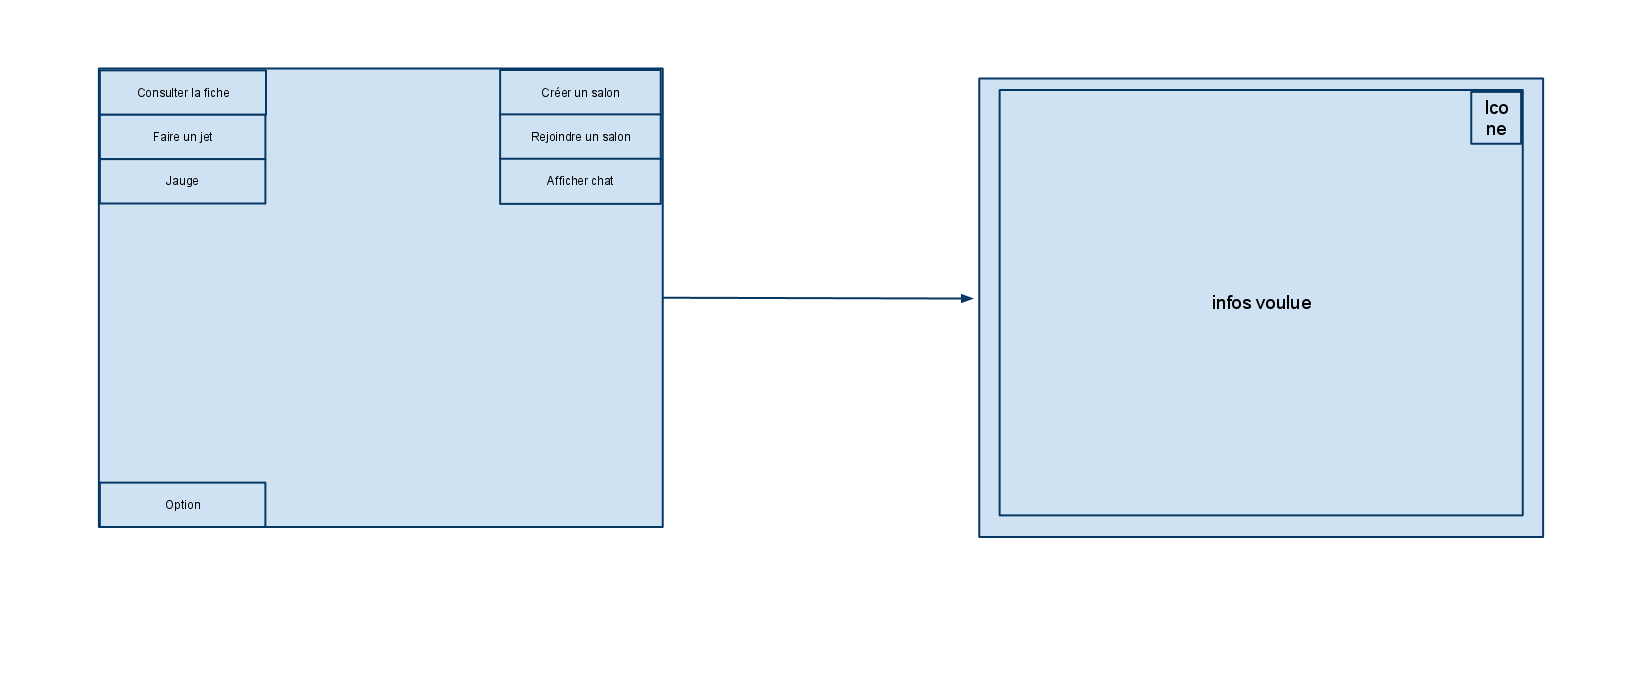
\includegraphics[height=14cm,width=15cm]{image/screen1.png}
  		\caption{Ecran démarrage/concept}
  		\label{screen1}
\end{figure}

Sur la capture \ref{screen1} on peut voir le concept général, avec le transfert
sur un écran suivant son choix, on ne souhaitait pas de surimpression des
écrans.

\begin{figure}[h]
  	
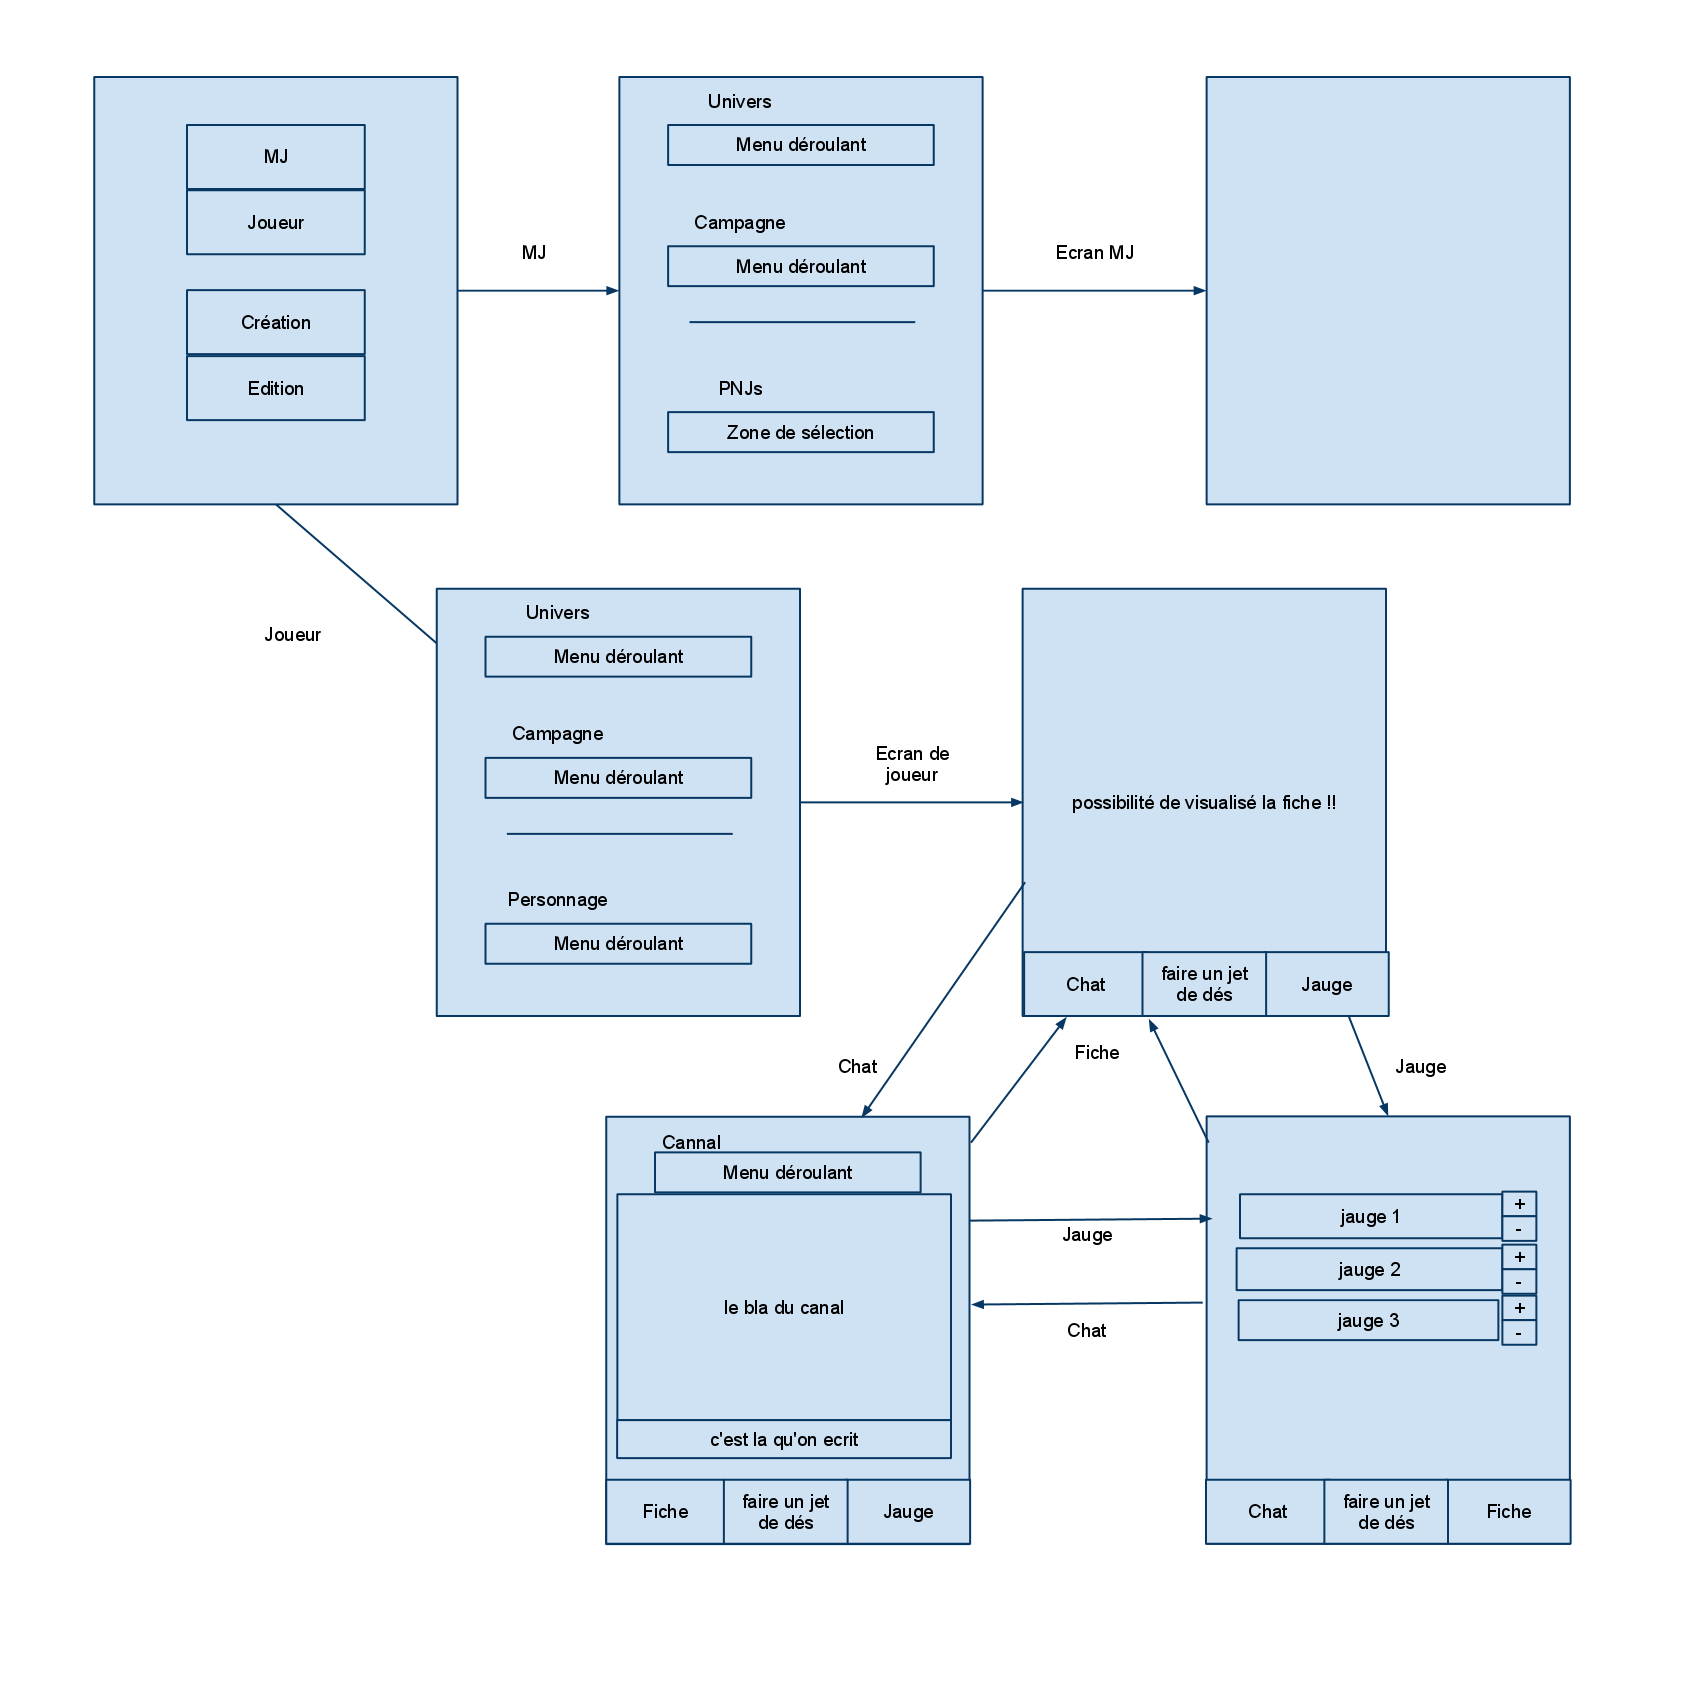
\includegraphics[height=14cm,width=15cm]{image/screen2.png}
  		\caption{Enchainement logique des écrans}
  		\label{screen2}
\end{figure}

La capture \ref{screen2} permet de voir plus en détail la logique d'enchainement
des écrans, avec l'affichage des fonctionnalités clés. Il montre aussi le fait
que l'on puisse basculer rapidement d'un écran à un autre. On voit aussi la
présence d'une partie jauge pour les éléments d'une fiche qui évoluent à chaque
instant du jeu. Ces éléments ne sont pas toujours regroupés dans une fiche et
se trouvent facilement dans notre application.

\begin{figure}[h]
  	
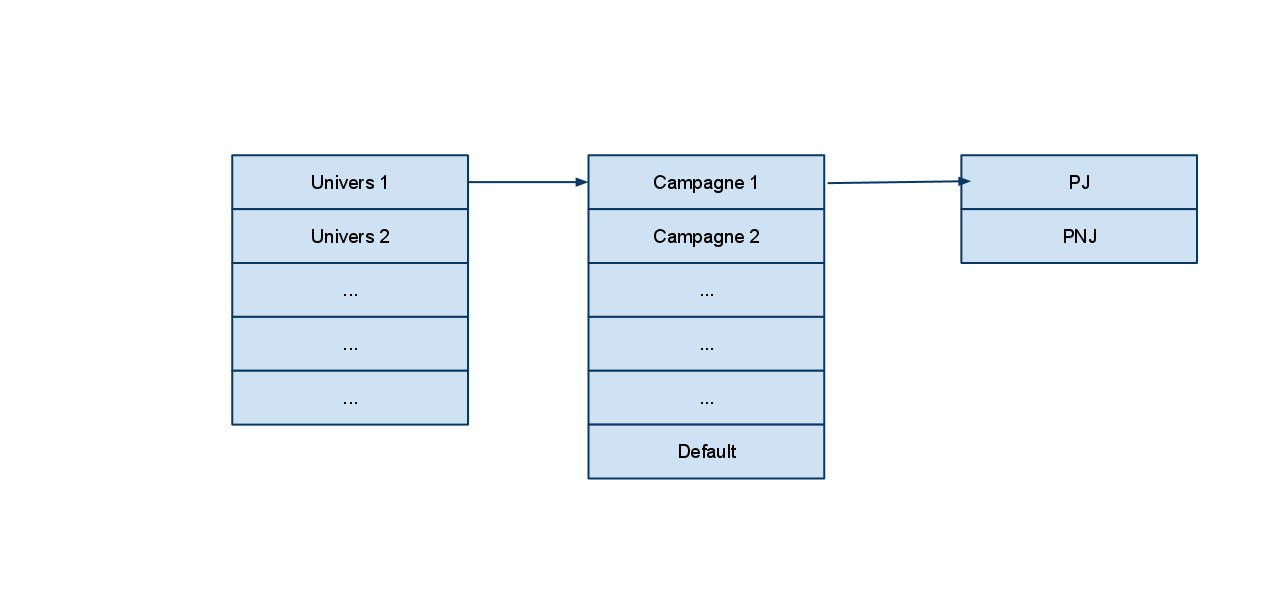
\includegraphics[height=10cm,width=15cm]{image/screen3.png}
  		\caption{Gestion des fiches}
  		\label{screen3}
\end{figure}

La capture \ref{screen3} montre la gestion des fiches de personnages en fonction
de l'univers (jeu en général), de la campagne, nom donné à un ensemble de
scénarios généralement cohérent dans lesquels évolue des personnages, une
histoire. Ensuite, une gestion des personnages joueurs et non joueurs pour un
meilleur tri des informations et un affinage des critères de sélections.

\begin{figure}[h]
  	
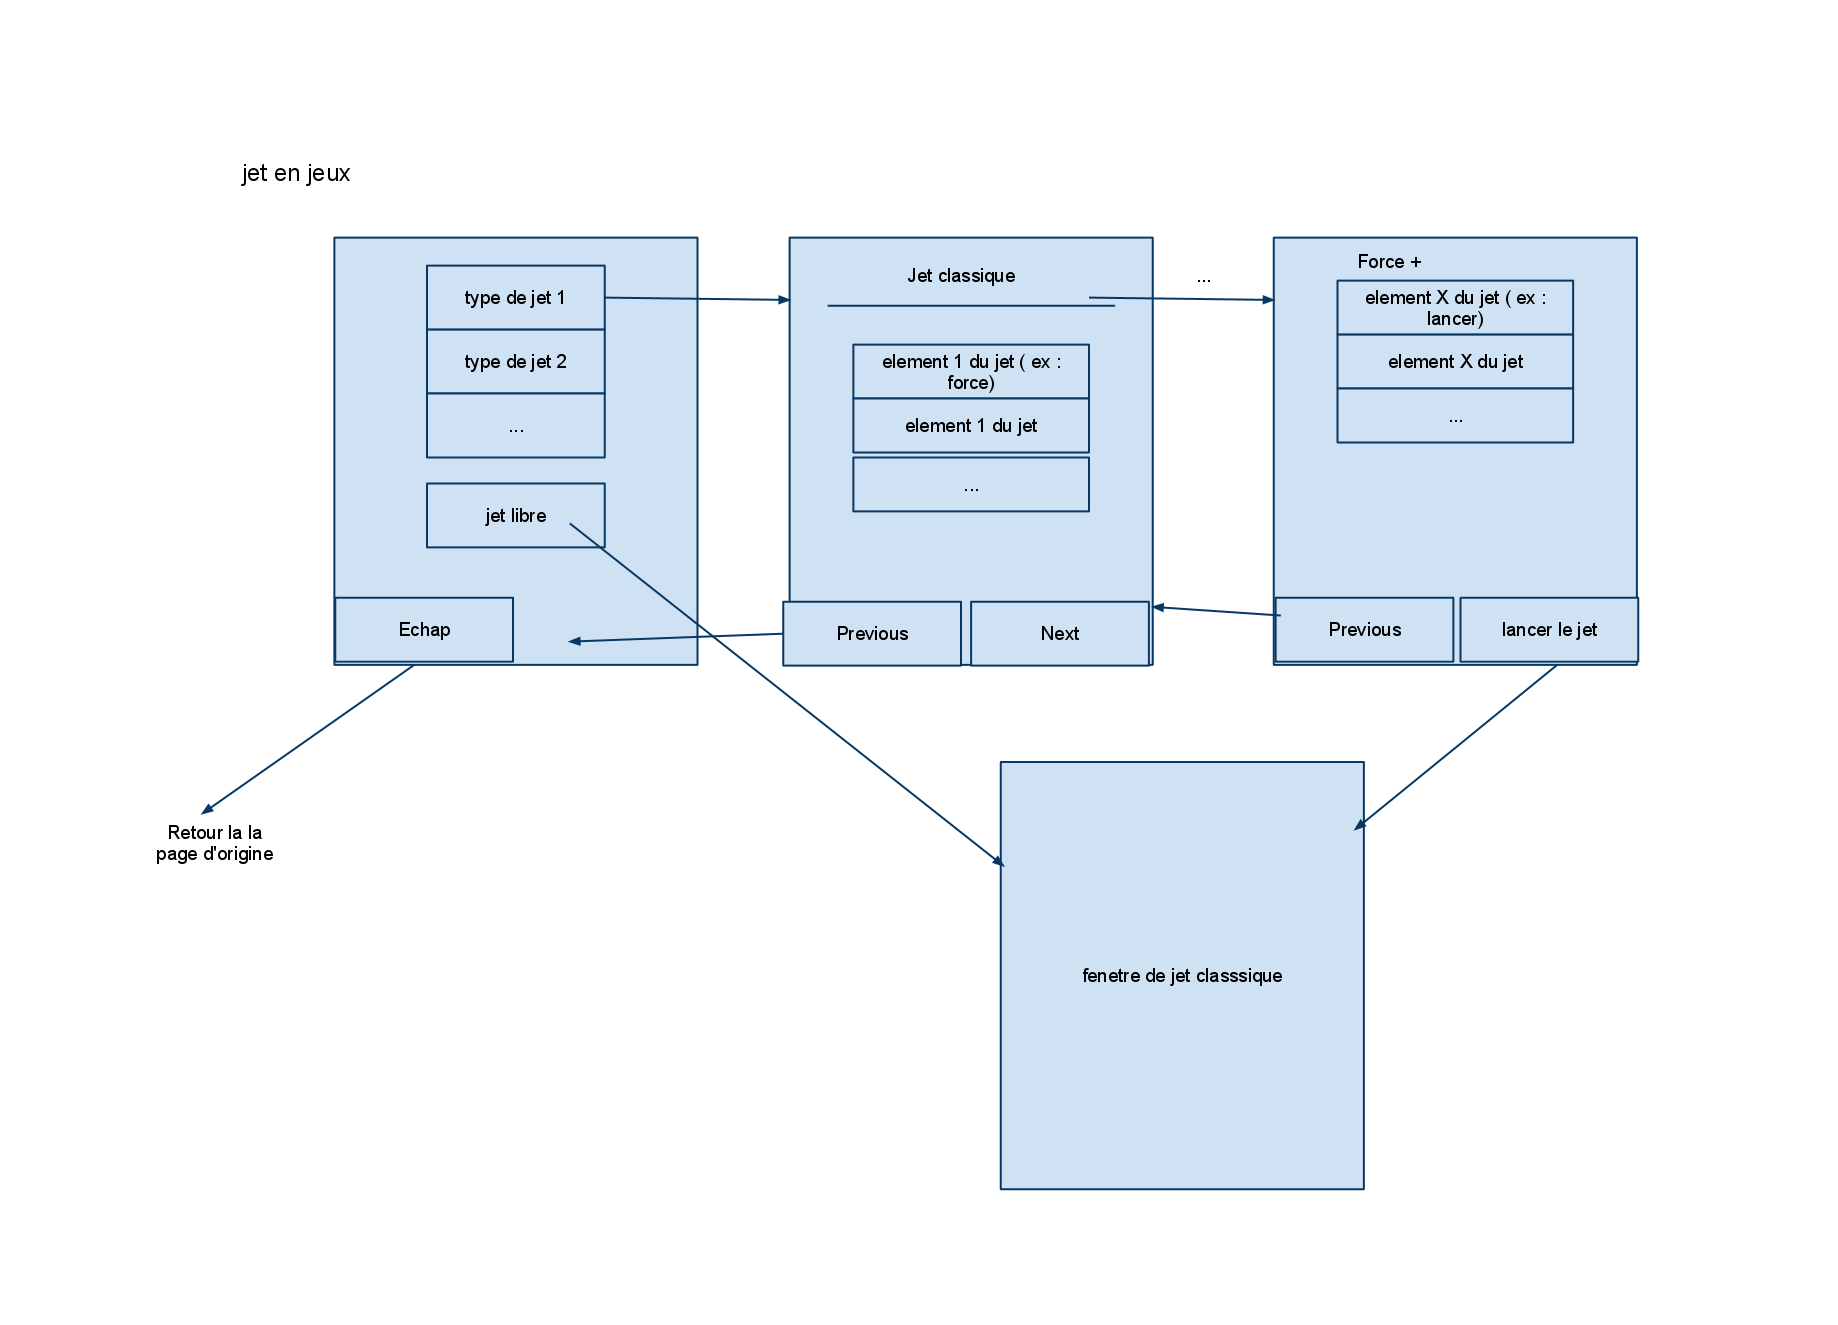
\includegraphics[height=10cm,width=12cm]{image/screen4.png}
  		\caption{Gestion des jets en jeu}
  		\label{screen4}
\end{figure}

La capture \ref{screen4} montre le choix du type du jet de dés, qui nous permet
de gérer en partie les règles d'un jeu et donc d'avoir des jets cohérents.
Ensuite, le joueur qui veut faire un jet choisit ses élements du jet.

\begin{figure}[h]
  	
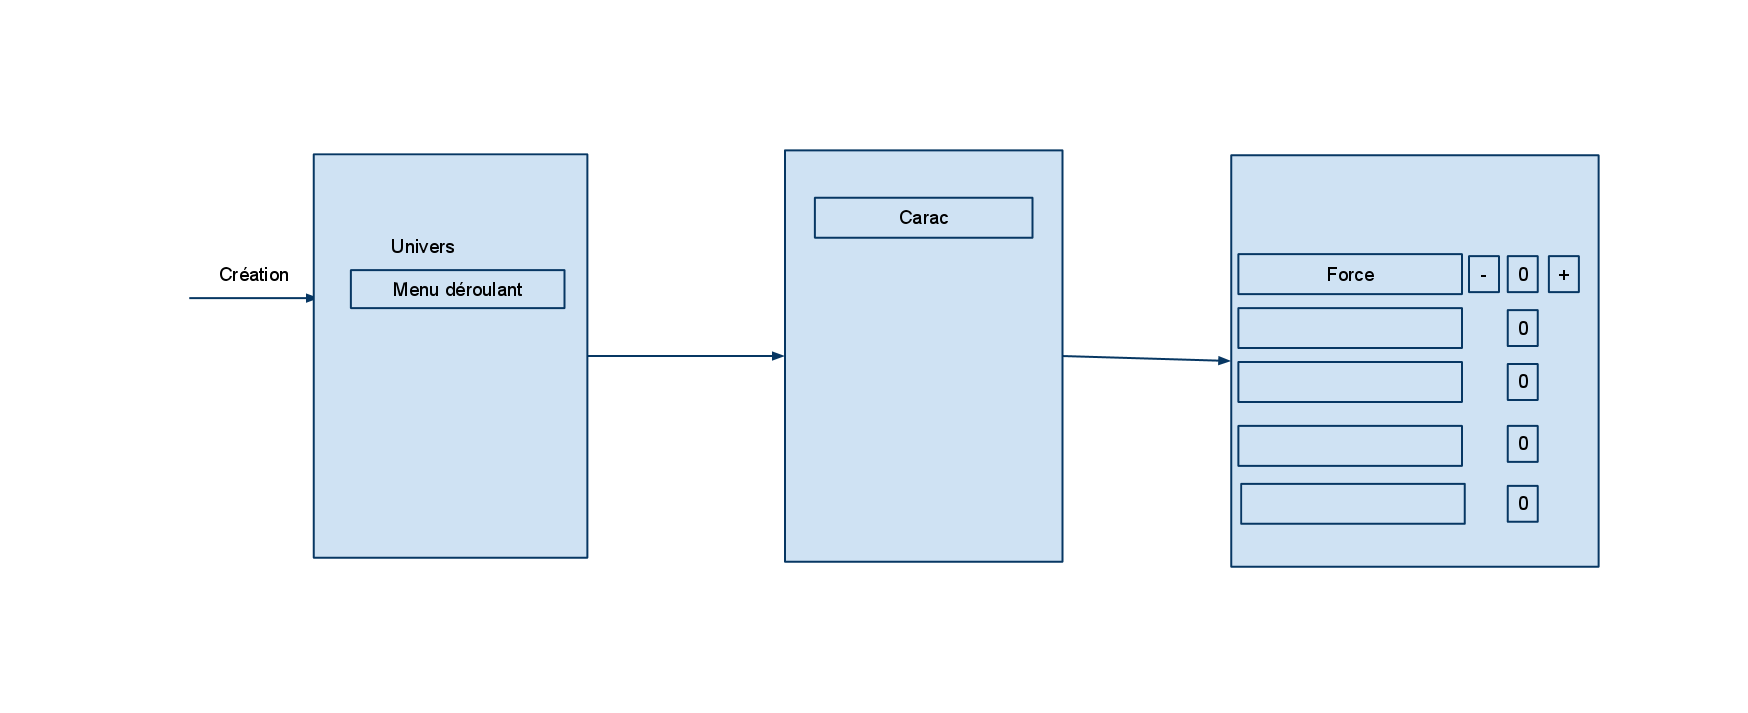
\includegraphics[height=12cm,width=15cm]{image/screen5.png}
  		\caption{Création de personnage}
  		\label{screen5}
\end{figure}

La capture \ref{screen5} nous montre la création de personnsage avec
l'affichage, des différents éléments de fiche à modifier à la création, l'écran
ne suppose aucune gestion de rêgle de création de personnage, et c'est le cas,
l'application ne supporte pas le rêgle de création.

\clearpage
\section{Lucid 4}

\subsection{Définition}

Cette étape de la méthode LUCID est une étape presque introspective, elle permet
de revenir sur les étapes précédentes par rapport au retour client sur le
prototypage. Et elle permet de commencer à établir le plan de construction de
l'application au niveau des fonctionnalités. Il s'agit de plannifier les tâches
de développement.

\subsection{Notre organisation}

Pour cette étape de la méthode, nous avons mis en parrallèle les
concepts initiaux du produit, les réactions et analyses des utilisateurs et les
esquisses. Nous avons pu faire remonter des remarques sur les premières
esquisses ainsi que nous rendre compte de ce qui était concrétement faisable
avec la plateforme android.

Cette étape à permis d'affiner clairement les fonctionnalités et de commencer à
appréhender la façon dont elles allaient exister concrétement sous une
plateforme mobile. Remettre à plat tout celà nous a permis de
dégager les étapes de développements que nous avions à faire.

Les travaux de définition et de modélisation des éléments liés au jeu de rôle a
été commune à tous les membres de l'équipe. La conception de modèle suffisamment
large pour assurer la prise en charge du plus de jeux possibles a été important.
Nous y avons tous participé puisque nous avions tous des expériences différentes
et qu'elles étaient relativement complémentaires.

Nous avons défini aussi l'architecture globale de l'application, architecture de
type composant, avec des composants comme:
\begin{itemize}
  \item Composant Dé
  \item Composant gestion des fiches en xml
  \item Composant connectivité(support bluetooh/wifi)
\end{itemize}

Ces composants censés être élémentaires doivent permettre la construction de
l'application. Nous avons appliqué le pattern adapter pour permettre
une éventuelle réutilisation de ces composants et surtout une relecture de code
plus aisée.

C'est pendant cette étape que nous avons choisi de ne pas implémenter la partie
connectivité de l'application. La méconnaissance du support androïd nous
ralentissant déjà pour les fonctionnalités plus simples.

Nous avons tous travaillé à enrichir nos connaissances sur androïd, en mettant
en place des petits tutoriels internes et en recoupant les informations
receuillies sur la plateforme.

De plus, pour travailler en collaboration nous avons choisi de mettre en place
un gestionnaire de version sous Google Code qui nous a accompagné tout au long
du developpement. De plus, nous avions des réunions régulières sur Skype pour
coordonnéer nos efforts de developpement. Enfin, nous utilisions en paralèlle
googledocs pour certains documents comme les esquisses.


\section{Lucid 5}

\subsection{Définition}

Cette étape de la méthode est l'implémentation de l'application. C'est donc dans
cette étape que l'interface est écrite en parrallèle avec le code effectif des
fonctions. C'est aussi le moment où l'on commence à écrire les documentations et
quelques structures communautaires autour de l'application. C'est vraiment à ce
moment que l'on rentre dans un cycle logiciel avec du concret informatiquement
parlant.

\subsection{L'implémentation}

Pour l'implémentation, il y a eu plusieurs phases mis en place. Tout d'abord, la
définition et l'écriture des composants en java sur lesquels l'application
devaient s'appuyer. Ce fut la première étape de developpement. Cette première
étape n'a pas forcément posé de problème au cours du projet.

Ensuite le développement s'est continué en s'appuyant sur ces premiers modules
de base.



\subsubsection{Modules de base}

Ces modules sont utilisés par l'interface graphique. Ils fournissent des
fonctionnalités propres au coeur de l'application.

\begin{itemize}
  \item DiceModule : il fournit différentes méthodes permettant d'effectuer
  plusieurs types de jet de dés.
  \item FicheModule : il permet d'enregistrer/charger une fiche de personnage à
  partir d'un modèle de fiche ou bien à partir d'une fiche même. Cela comprend
  aussi le parseur xml nécessaire à ces opérations.
  \item SystemModule : idem que FicheModule mais pour un système de règles.
\end{itemize}

\subsubsection{IHM Android}

Pour expliciter notre interface androïd, nous avons fait le choix d'expliquer
les types d'écran utilisés et non chacun d'eux afin d'être plus synthétique.

\paragraph{Interface à boutons}
~\\
~\\
 Ce type d'interface est utilisé dans la page d'accueil de notre application.
 Il permet un choix simplifié pour l'utilisateur.

\paragraph{Interface avec listeView}
~\\
~\\
Nous avons utilisé les listView dans des écran de sélection. Celui-ci est rempli
dynamiquement avec du texte provenant du parsing de fiche ou d'un système de
règles. Chaque élément est cliquable afin d'avancer dans le processus
d'application. Par exemple, la sélection d'un des éléments d'un jet de dé.\\

De plus, nous avons utilisé cet outil graphique afin de modifier des valeurs
associées par exemple à des compétences. Nous avons donc personnalisé chaque
ligne de la listView à l'aide d'un Adapter. Cette ListView ne comprend donc
plus uniquement du texte mais des boutons ou encore des EditText.

\paragraph{Interface avec Spinner}
~\\
~\\
L'utilisation des Spinners a été nécessaire pour faciliter les choix de
l'utilisateur. Ces Spinners permettent une sélection filtrées des univers et des
campagnes. Par exemple, lorsque l'utilisateur veut voir une fiche, il
sélectionne dans un premier temps l'univers. Puis, il sélectionnera les
différentes campagnes disponibles par rapport à cet univers et enfin les fiches
disponibles pour cet univers et cette campagne.

\paragraph{Interface du jet de dé}
~\\
~\\
Ce type d'interface permet d'effectuer un jet de dé utilisant différents outils
graphiques androïd. Soit en le paramétrant totalement, soit après avoir
sélectionné les différents éléments du jet.

\section{Lucid 6}

\subsection{Définition}

Cette étape de la méthode est l'évaluation externe du projet. Elle s'accompagne
généralement de la diffusion d'une première version public du produit qui
normalement, est proche de la version finale tant par l'aspect que par ses
fonctionnalités.
Cette étape permet de lever les dernières remarques du public visé et de
corriger les bugs induits par la différence d'utilisation de chaque personne par
rapport à l'utilisation des developpeurs.


\subsection{Plan d'évalution}

Pour l'évalutation de notre application, nous avons pensé à plusieurs niveaux
d'écoute des utilisateurs. Nous proposons une application qui se veut pour un
large panel de joueurs et de MJ avec des attentes différentes.

Nous avons pensé à trois niveaux d'évaluation par les utilisateurs ou trois
types de niveaux de communication avec la communauté. Un pour les MJ,
utilisateur amené à faire évoluer les modèles de fiches et les contraintes
d'affichage pour information multiple.

Un autre pour les "simples" utilisateur, client/consommateur voulant s'en servir
pour se séparer du support physique pour plus de facilité. La synchronisation de
fiche, édition, jeu, jets de dés etc. De plus, pour ce "niveau", l'écoute de
joueurs avancés ayant dépassés la phase d'apprentissage du média sera
importante pour une ergonomie optimale de l'application.

Enfin, le dernier type correspondrait aux retour des utilisateurs ne maîtrisant
que peu le support androïd. Ceux-ci représentent une cible privilégié sur le
retour, le but étant d'être particulièrement à l'écoute de ces utilisateurs. En
effet, pour leur permettre de bien prendre en main l'application, nous devons
mettre en place un apprentissage efficace pour faire d'eux des utilisateurs
"simple".

Le but final est un nivellement du niveau des utilisateurs vers le niveau
simple, ou tout du moins qu'à terme il n'y ait que deux niveaux d'utilisateur.
C'est-à-dire que tout utilisateur novice devienne rapidement un utilisateur
simple pour qu'il puisse profiter pleinement de l'application. En effet, si
l'utilisation de l'application le ralentit lors d'une partie cela irait à
l'encontre des objectifs de l'application.

Un des avantages à être sur une plateforme tactile c'est que l'aprentissage est
assez rapide et simple pour peu que l'application ait bien été construite, ce
que nous espérons dans notre cas.

\clearpage
\section{Conclusion}

Lucid est une méthode résolument ethno-centré, c'est un fait indéniable et nous
l'avons constaté du fait de la proximité nécessaire avec les futurs
utilisateurs. C'est un avantage certain pour l'acceptation finale du produit par
l'utilisateur.

Le reproche que l'on pourrait faire serait que cette méthode par certains
aspects, entre en conflit avec les méthodes d'ingénierie logicielle classique. 
Bien qu'il y ait des similitudes, il y a quelques incompatiblités entre ces
deux méthodes.

On gagne pourtant à utiliser LUCID, on a  plus de chance que le produit soit
accepté et conforme à ce que l'utilisateur final va vouloir. Cependant, le temps
nécessaire plus long qu'un cycle "classique" implique potentiellement plus
d'argent à investir pour le client. L'idéal serait une méthode de developpement
intégrant l'ethno-centrisme de LUCID avec la performance de d'autres méthodes.

Un autre soucis que l'on peut remarquer avec LUCID c'est l'aspect communication
avec le client, allant de paire avec l'analyse de ses besoins et la
transcription en élément informatique concret et utilisable. Cet aspect social,
la communication des développeurs avec les clients est généralement compliquée.
Or, actuellement, les clients ne prennent pas souvent le temps de parler avec
l'équipe de développement et le marché des informaticiens est saturé par des
gens associaux qui ont naturellement des problèmes de communication!

En conclusion, cette méthode est très intéressante mais peut-être trop utopiste
compte tenu de la situation actuelle.


  
  
\end{document}

